\chapter{CONCEITOS E TÉCNICAS NECESSÁRIAS}

O capitulo explica termos técnicos essenciais para o melhor entendimento do trabalho.

\section{Samba}

Samba é um software \textit{open source} que provê serviços a clientes nos protocolos SMB e CIFS.
O samba permite a interoperabilidade entre servidores Linux/Unix e clientes baseados na
plataforma Windows.
O samba permite que um servidor linux seja apto a fornecer serviços como:
  \begin{itemize}
    \item \textbf{\#Servidor de arquivos e impressão} Utilizando o protocolo \textit{Server Message Block} para possibilitar o compartilhamento de arquivos, pastas volumes e impressoras na rede.

    \item \textbf{\#Autenticação e autorização} Identifica um computador ou um usuário da rede e determina os direitos de acesso a arquivos que cada usuário possui, através de tecnologias como permissões de arquivos, diretivas de grupo e o serviço de autenticação Kerberos.

    \item \textbf{\#Resolução e busca de nomes e diretórios} Compartilha as principais informações sobre computadores e usuários da rede através do \textit{LightWeight Directory Access Protocol} (LDAP).% e o Microsoft Active Directory.

    \item \textbf{\#Servidor de domínio como PDC} Funcionando como controlador de domínio ativo dentro de um domínio Windows.
  \end{itemize}

Basicamente, o Samba é um servidor e um conjunto de ferramentas que permite o compartilhamento de arquivos e impressoras sistemas Windows e Linux. Usando o Samba em um servidor Linux, ele se comporta exatamente como um servidor Windows, podendo inclusive autenticar usuários e compartilhar impressoras. Outra característica do Samba é que ele pode atuar como um Controlador Primário de Domínio (PDC), armazenando perfis de usuários, realizar controle de acesso, sendo suas as configurações tão efetivas quanto às de um servidor Windows \cite{FOCA}.

%\section{Permissões no Linux}

\section{Permissões especiais no Linux}

Existe no Linux três permissões especiais, para dar segurança ao sistema, chamadas assim por somente serem atribuídas a arquivos específicos (arquivos executáveis e diretórios). Tais permissões são fornecidas pelos bits SUID, SGID e STICKY.

  \begin{itemize}
    \item \textbf{\#SUID} O bit SUID (Set UID) é aplicável apenas a arquivos executáveis, fazendo com que estes rodem com as permissões de seu proprietário, independente de quem tenha executado-o. Pode ser útil para que usuários comuns possam executar arquivos permitidos apenas a administradores.

    \item \textbf{\#SGID} O bit SGID (Set GID) pode ser aplicado a um arquivo executável e a um diretório. No primeiro caso ele tem as mesma função do SUID, porém rodando com as permissões de um grupo de usuários. No segundo, ele força os arquivos e diretórios criados dentro do diretório pai (o que obteve a permissão) a pertencerem ao mesmo grupo, independente do grupo de quem tenha-os criado.

    \item \textbf{\#STICKY} O bit STICKY é aplicável a diretórios e faz com que a exclusão de arquivos pertencentes a estes diretórios seja apenas permitida ao dono do arquivo e ao administrador do sistema. Tem vantagem sobre a permissão “Somente Leitura” no diretório pois faz com que outros usuários possam criar e editar qualquer arquivo, impedindo-os apenas de apagá-lo.
  \end{itemize}

\section{PDC}

O Controlador de Domínio é responsável por fornecer autenticação para os clientes,sejam sistemas Linux ou Windows. Ou seja, apenas centraliza contas de usuários e fornece recursos voltados para a administração de usuários, como a gestão de perfis móveis, que são as configurações de usuários que são lidas, independente de qual máquina o usuário utilize.Em uma rede de com pouco mais de 10 clientes a necessidade de ter um PDC é mais aparente,pois fica cada vez mais difícil de gerenciar as contas de clientes e máquinas conforme o crescimento da rede. Com o Controlador de Domínio também é possível fornecer acesso por perfis móveis onde o usuário pode ter acesso à sua área de trabalho independente da máquina (da mesma rede) onde faz o login. Em contrapartida, bloqueando uma conta de usuário,automaticamente este estará bloqueado em todas as máquinas gerenciadas pelo Controlador de Domínio \cite{MORIMOTO}

\section{NETBIOS}

NETBIOS, \textit{Networking Basic Input/Outbut System}, é uma API desenvolvida em 1984 pela IBM, que fornece serviços relacionados na camada de sessão do modelo OSI, permitindo a comunicação entre computadores na rede através de um nome NETBIOS correspondente a um \textit{hostname}.\cite{WIKIPEDIA}

\begin{figure}[ht]
   	\centering
    \scalebox{1}{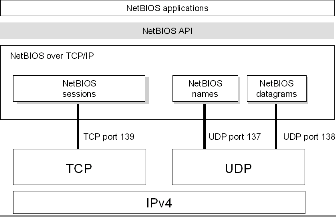
\includegraphics{figuras/netbios}}
   	\caption{Estrutura do funcionamento da NetBios \cite{NETBIOS}}
    \label{netbios}
\end{figure}

% \section{Domain Master}
% 
% ***VERIFICAR REFERENCIA***
% 
% DOMAIN MASTER BROWSER Uma vez que o Local Master Browser é eleito no segmento de rede, uma consulta é feita ao servidor WINS para saber quem é o Domain Master Browser da rede para enviar a lista de compartilhamentos. A máquina escolhida como Local Master Browser envia pacotes para a porta UDP 138 do Domain Master e este responde pedindo a lista de todos os nomes de máquinas que o Local Master conhece e também o registra como Local Master para aquele segmento de rede.

% \section{WINS}

%\textit{Windows Internet Name Service} (WINS) ou \textit{NetBIOS Name Services} (NBNS) é um serviço do protocolo TCP/IP. Este serviço faz a resolução nomes e números IP e os armazena, disponibilizando esta informação para quem necessite usar. Cada cliente envia seu nome NetBIOS e número IP para o servidor WINS, que armazena estas informações em um banco de dados. Quando um cliente desejar se comunicar com um outro, ele envia o nome desejado ao servidor WINS. Se o nome constar na base de dados, o servidor WINS retorna ao solicitante o número IP.

%O WINS não é mais necessário, pois hoje tem os servidores DNS e o WINS só se faz necessário para manter a compatibilidade com Windows Antigos.

\section{\textit{Active Directory}}

O \textit{Active Directory} (AD) é um serviço de diretório nas redes Windows 2000 e 2003.

Serviço de diretório é um conjunto de Atributos sobre recursos e serviços existentes na rede, isso significa que é uma maneira de organizar e simplificar o acesso aos recursos de sua rede centralizando-os; Bem como, reforçar a segurança e dar proteção aos objetos da base de dados contra intrusos, ou controlar acessos dos usuários internos da rede.

O \textit{Active Directory} mantém dados como contas de usuários, impressoras,grupos,computadores, servidores,recursos de rede, etc. Ele pode ser totalmente escalonável, aumentando conforme a nossa necessidade.\cite{LOSANO}

\section{DNS}

DNS (\textit{Domain Name System}) é uma base de dados hierárquica e distribuída, usada para a resolução de nomes de domínios em endereços IP. É considerado como um banco de dados distribuído que converte nomes de \textit{hosts} (máquinas) para endereços IP. É basicamente um mapeamento de endereços IP e seus respectivos nomes. A utilização mais comum é na internet. Todos os computadores da rede possuem um endereço IP. Os servidores DNS simplesmente transformam ou resolvem esse o número em um nome. Por exemplo, o endereço www.iff.edu.br corresponde ao IP 200.143.198.110. \cite{SCRIMER}

\begin{figure}[ht]
   	\centering
    \scalebox{1}{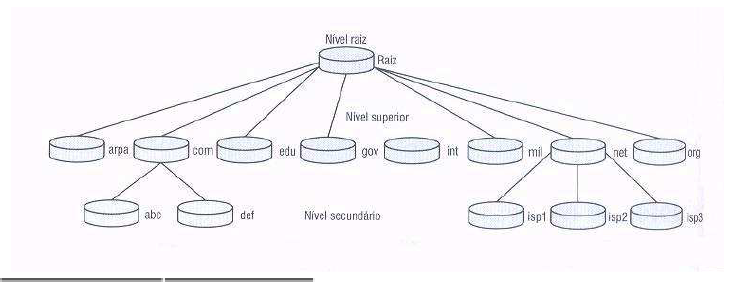
\includegraphics{figuras/dns}}
   	\caption{Estrutura hierárquica do DNS \cite{SCRIMER}}
    \label{dns}
\end{figure}

\section{BIND}


BIND (\textit{Berkeley Internet Name Domain} ou, como chamado previamente, Berkeley Internet Name Daemon) é o servidor para o protocolo DNS mais utilizado na Internet, especialmente em sistemas do tipo Unix, onde ele pode ser considerado um padrão de facto. Foi criado por quatro estudantes de graduação, membros de um grupo de pesquisas em ciência da computação da Universidade de Berkeley, e foi distribuído pela primeira vez com o sistema operacional 4.3BSD. O programador Paul Vixie, enquanto trabalhava para a empresa DEC, foi o primeiro mantenedor do BIND. Atualmente o BIND é suportado e mantido pelo \textit{Internet Systems Consortium}.
Para a versão 9, o BIND foi praticamente reescrito. Ele passou a suportar, dentre outras funcionalidades, a extensão DNSSEC e os protocolos TSIG e IPv6 \cite{BIND}.

\section{LDAP}

O LDAP (\textit{Lightweight Directory Access Protocol}) é o protocolo responsável por fornecer Serviço de Diretórios a computadores Windows de forma similar ao \textit{Active Directory} da Microsoft, que é baseado no LDAP. Tais serviços incluem conexões de computadores, grupos de computadores, usuários, administração de identidades, além de possibilitar uma maneira eficiente de descrever, localizar e administrar esses recursos.

LDAP é um protocolo para acessar informações contidas em um diretório. Por ser um protocolo cliente/servidor o LDAP permite navegar, ler, armazenar e pesquisar informações e realizar tarefas de gerenciamento em um serviço de diretórios. O serviço de diretório é um banco de dados otimizado para leitura,navegação e pesquisas \cite{TRIGO}.

\begin{figure}[ht]
   	\centering
    \scalebox{1}{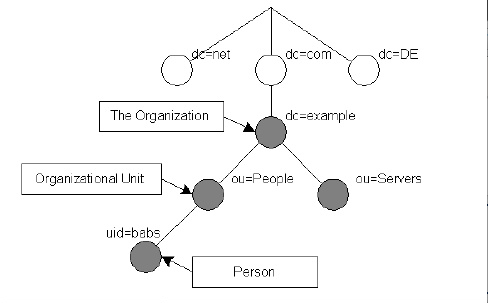
\includegraphics{figuras/ldap}}
   	\caption{Estrutura do protocolo LDAP \cite{LDAP}}
    \label{ldap}
\end{figure}

\section{Kerberos}

Kerberos é um protocolo de segurança de rede e fornece autenticação entre computadores e usuários através de um servidor centralizado que concede autenticações criptográficas a qualquer computador utilizando o Kerberos. Esse sistema de segurança e autenticação agraga diversos benefícios como autentificação mútua, autentificação delegada, interoperabilidade e gerência simplificada e confiável. O samba pode usar o Kerberos como um mecanismo autenticação de computadores e usuários.

O Kerberos é um protocolo que prevê forte autenticação entre aplicações cliente-servidor e usa criptografia de chave simétrica no qual servidores fornecem acesso aos serviços solicitados pelos clientes, caso provem que são eles mesmos. \cite{FILHO}

%O Kerberos não autentica o host no servidor, apenas a aplicação que oferece o serviço.Ele trabalha com tickets , servindo para provar a autenticidade de um usuário e garantir oacesso aos serviços e aplicações. (CONECTIVA, 2009).

%Quando um usuário entra com as informações de login , considerando que seja umusuário cadastrado no KDC (é o servidor Kerberos), os dados são enviados para o servidor 25Kerberos que recebe as informações e as confere com as que estão cadastradas no banco dedados. Estas informações são criptografadas com a própria senha do usuário e enviadas devolta para ele. Este é o ticket TGT (Ticket-Grant-Ticket). Se as informações do ticket TGTpuderem ser descriptografadas, então o usuário é quem diz ser. O TGT é armazenado namáquina e, por segurança, tem um tempo de vida útil para o caso de ser interceptado na rede.(CONECTIVA, 2009)
 
\begin{figure}[ht]
   	\centering
    \scalebox{1}{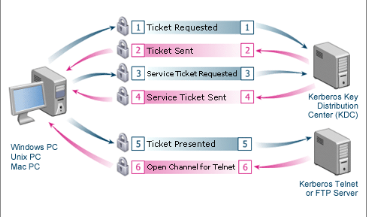
\includegraphics{figuras/kerberos}}
   	\caption{Autenticação Kerberos \cite{KERBEROS}}
    \label{kerberos}
\end{figure}
figura 7 - Autenticação Kerberos \cite{KERBEROS}

%\section{NTP}

%Os servidores NTP permitem aos seus clientes a sincronização dos relógios de seus computadores e outros equipamentos de rede a partir de uma referência padrão de tempo aceita mundialmente, conhecida como UTC (\textit{Universal Time Coordinated}).\cite{RNP}

%\section{NTVFS}

%Sistema de arquivos que armazena os atributos do NTFS

\section{GSSAPI}

A GSSAPI é uma interface que permite desenvolvedores escreverem aplicações que aproveitam mecanismos de segurança tais como Kerberos, sem ter de programar explicitamente para qualquer mecanismo, ou seja, aplicações genéricas do ponto de vista de segurança. Programas que usam GSSAPI são, deste modo, altamente portáteis, não somente de uma plataforma para outra, mas de uma configuração de segurança a outra e de um protocolo de transporte a outro. A GSSAPI fornece vários níveis de proteção de dados, consistentes com os mecanismos de segurança subjacentes.\cite{HUGO}


%\section{Referencias - Temporário}

% SAMBA:
% http://pt.wikipedia.org/wiki/Samba\_(servidor)
% 
% http://en.wikipedia.org/wiki/Samba\_(software)
% 
% http://www.samba.org/samba/docs/
% 
% http://www.samba.org/samba/what\_is\_samba.html
% 
% http://www.samba.org/samba/docs/SambaIntro.html
% 
% http://www.samba.org/cifs/docs/what\-is\-smb.html
% 
% http://www.samba.org/cifs/
% 
% Using Samba (OREILLY)
% 
% NETBIOS:
% 
% http://pt.wikipedia.org/wiki/Netbios
% 
% Using Samba (OREILLY)
% 
% SMBD: 
% 
% Using Samba (OREILLY)
% http://www.samba.org/samba/docs/
% 
% NMBD:
% 
% Using Samba (OREILLY)
% http://www.samba.org/samba/docs/

%POSTFIX.ORG.BR. Disponível em: http://www.postfix.org/LDAP\_README.html\# config.Acesso em dezembro de 2009.

%SAMBA.ORG-1.Samba4 / Active Directory. Disponível em:http://wiki.samba.org/index.php/Samba4/ActiveDirectory. Acesso em: dezembro de 2009

%SAMBA.ORG-2.Apresenta informações sobre schemas e ldap. Disponível em:http://wiki.samba.org/index.php/Samba4/LDAP\_Backend. Acesso em dezembro de 2009.

%SAMBA.ORG-3. Instalação e configuração do Samba 4. Disponível em:http://wiki.samba.org/index.php/Samba4/HOWTO\#Step\_1:\_download\_Samba4. Acessoem outubro de 2009.

%Apresenta funcionamento do protocolo CIFS. Disponível em:http://www.gta.ufrj.br/grad/01\_2/samba/smbcifsinternamente.htm. Acesso em outubro de2009.

%Ldap Browser. Versão 2.6. Softerra. 2004.

%ALECRIN. E. Servidor Samba: o que é. Disponível em:http://www.infowester.com/linuxsamba.php. Acesso em dezembro de 2009.


%ERICH. S. M.Autenticação Integrada Baseada em Serviço de Diretório LDAP. Apresentaestudo do protocolo LDAP. Disponível em http://www.linux.ime.usp.br/~cef/mac499-06/monografias/erich/html/ch01s05.html. Acesso em dezembro de 2009

%FILHO.M.M.C. Kerberos. Apresentação do protocolo Kerberos. Disponível em:http://www.gta.ufrj.br/grad/99\_2/marcos/kerberos.htm. Acesso em julho de 2009

%FOCA GNU/Linux. Samba. Disponível em: http://www.guiafoca.org/guia/avancado/ch-s-samba.htm. Acesso em novembro de 2009.

%LDAP.ORG.BR Como instalar um PDC Samba+OpenLDAP. Disponível em:http://www.ldap.org.br/modules/ldap/files/files///samba+openLDAP+qmail.pdf. Acessoem setembro de 2009.

%Linux Magazine. São Paulo. Linux New Media do Brasil Editora Ltda. 2009. Mensal. ISSN1806-9428.

%LOSANO.M. Introdução ao Active Directory. Apresenta visão geral do Active Directory.Disponível em: http://technet.microsoft.com/pt-br/library/cc668412.aspx. Acesso emagosto de 2009.

%MICROSOFT-1. Simple Network Time Protocol. Apresenta detalhes do protocolo SNTP.Disponível em: http://msdn.microsoft.com/pt-br/library/aa919019.aspx. Acesso emagosto de 2009

%MICROSOFT-2. Descrição dos protocolos do Active Directory. Disponível em:http://technet.microsoft.com/pt-br/library/cc961766\%28en-us\%29.aspx. Acesso emsetembro de 2009.

%MINASI. M; ANDERSON. C.;SMITH. B.M;TOOMBS.D. Dominando o Windows 2000Server. São Paulo. Pearson Education do Brasil. 2001. 1275 p.

%MICROSOFT-3. Apresenta as operações mestres do Active Directory. Disponível emhttp://technet.microsoft.com/pt-br/library/cc716426.aspx. Acesso em dezembro de 2009.

%MORIMOTO.C.E. Redes e Servidores Linux - Guia Prático. Porto Alegre. Sul. 2005. 302p.